\chapter{Các kết quả thí nghiệm}
\label{Chapter4}

% \noindent\textit{Trong chương này, nhóm chúng em trình bày các kết quả thí nghiệm để đánh giá các đề xuất tìm hiểu được từ bài báo đã được nói ở chương trước. Bộ dữ liệu được dùng để tiến hành thí nghiệm là bộ COAT (bao gồm đánh giá của người dùng cho áo khoác), bộ Yahoo (bao gồm đánh giá của người dùng cho các bài hát), bộ Movielens 100K (bao gồm đánh giá của người dùng cho các bộ phim). Các kết quả thí nghiệm cho thấy khi khi dùng IPS đánh giá mô hình hoàn toàn khớp với hiệu suất thật và tốt hơn nhiều so với các độ đo đánh giá truyền thống. Các kết quả thí nghiệm cũng cho thấy mô hình được huấn luyện dựa trên độ đo IPS cũng cho kết quả tổng quát hóa tốt hơn trên các mức độ selection bias khác nhau.}

\section{Các thiết lập thí nghiệm}
\label{sec:4_setup}
\subsection{Các tập dữ liệu}
Nhóm chúng em sẽ tiến hành các thí nghiệm về hiệu năng của mô hình ``Matrix factorization'' truyền thống (MF) so với ``Matrix factorization'' sử dụng độ đo IPS (MF-IPS). Các thí nghiệm về hiệu năng này sẽ được đánh giá trên 2 tập dữ liệu Coat Shopping và Yahoo!R3, 2 tập dữ liệu này đều có tập training bị thiên lệch dữ liệu do người dùng tự lựa chọn chọn sản phẩm để đánh giá; và có một tập test không bị thiên lệch do người dùng đánh giá một tập các sản phẩm ngẫu nhiên. Thông tin cụ thể của từng tập dữ liệu được mô tả như sau:
\begin{itemize}
    \item Tập dữ liệu Coat Shopping: tập dữ liệu này chứa đánh giá của các người dùng cho các áo khoác, được thu thập bằng cách mô phỏng dữ liệu bị thiên lệch của những người dùng mua áo khoác trong cửa hàng trực tuyến. Những người dùng được yêu cầu phải đánh giá 24 chiếc áo khoác họ tự chọn và 16 chiếc áo khoác được chọn ngẫu nhiên theo phân phối đều dựa trên thang điểm từ 1 đến 5. Tập dữ liệu chứa đánh giá từ 290 người dùng cho 300 sản phẩm. Các điểm đánh giá do người dùng tự lựa chọn sẽ được sử dụng làm tập huấn luyện, đồng thời, các điểm đánh giá trên tập các sản phẩm ngẫu nhiên sẽ được dùng để kiểm tra. 
    \item Tập dữ liệu Yahoo!R3: tập dữ liệu này chứa đánh giá của các người dùng cho các bài hát. Tập dữ liệu huấn luyện bị thiên lệch cung cấp hơn 300 nghìn đánh giá cho các bài hát, các bài hát này được tự lựa chọn bởi 15400 người dùng. Tập dữ liệu kiểm tra chứa đánh giá của 5400 người dùng cho 10 bài hát được chọn ngẫu nhiên theo phân phối đều.
\end{itemize}

Ngoài ra, nhằm đánh giá ảnh hưởng của việc dữ liệu bị thiên lệch tới việc học của MF và MF-IPS nhóm chúng em còn tiến hành thí nghiệm trên tập dữ liệu MovieLens 100k. Tập dữ liệu này chứa đánh giá của các người dùng cho các bộ phim. Tập dữ liệu MovieLens 100k sẽ chứa 100 000 đánh giá (từ 1 đến 5) của 943 người dùng trên 1682 bộ phim, trong đó mỗi người dùng sẽ đánh giá ít nhất 20 bộ phim. Các bộ phim được đánh giá trong tập dữ liệu này đều do người dùng tự lựa chọn, vì vậy đây là một tập dữ liệu bị thiên lệch. Do đó để thí nghiệm về ảnh hưởng của dữ liệu bị thiên lệch nhóm chúng em sẽ tiến hành tạo một bộ dữ liệu MovieLens 100k giả lập dựa trên bộ dữ liệu gốc, cách tạo bộ dữ liệu giả lập này sẽ được nhóm chúng em giới thiệu cụ thể trong phần \ref{subsubsection:MovieLens}.

\subsection{Các thiết lập về huấn luyện và kiểm tra}
Trong tất cả các thí nghiệm, nhóm chúng em sẽ tiến hành lựa chọn các siêu tham số regularization $\lambda$ và tham số đặc trưng tiềm ẩn $d$ cho mô hình ``Matrix factorization'' thông qua phương pháp ``k-fold Cross-Validation'' với $k=4$. Cụ thể, phương pháp ``k-fold Cross-Validation'' sẽ tách tập dữ liệu quan sát được MNAR thành 4 phần bằng nhau, trong đó 3 phần sẽ được sử dụng như là tập training và 1 phần còn lại sẽ được sử dụng như là tập validation để đánh giá mô hình huấn luyện được. Do tập dữ liệu được chia thành 4 phần vì vậy các propensity cũng cần được điều chỉnh cho phù hợp; cụ thể ở tập training, propensity sẽ được nhân với $\frac{3}{4}$ và ở tập validation propensity sẽ được nhân với $\frac{1}{4}$. Các tham số cho độ lỗi nhỏ nhất khi đánh giá trên tập validation sẽ được sử dụng để huấn luyện lại trên toàn bộ tập dữ liệu quan sát được. 

Để đánh giá hiệu năng của mô hình, nhóm chúng em sẽ sử dụng độ đo Mean square error (MSE) để đánh giá độ lỗi của giá trị dự đoán của mô hình so với tập test. Độ lỗi trên 2 tập dữ liệu Coat và Yahoo sẽ được tính toán thông qua tập test được cung cấp sẵn. Còn đối tập dữ liệu Movielens 100k, độ lỗi sẽ được tính toán dựa trên dữ liệu giả lập.


\section{Kết quả cài đặt của nhóm chúng em so với kết quả cài đặt của bài báo}
Đầu tiên, nhóm em tiến hành thử nghiệm để xem hiệu quả của phương pháp học MF-IPS so với phương pháp MF thông thường trên hai bộ dữ liệu thế thới thực là Coat và Yahoo!R3. Trên bộ dữ liệu Coat, nhóm em sử dụng phương pháp ``Logistic Regression'' để ước lượng ma trận propensity như đã trình bày ở phần \ref{sec:3_estimate_LR}, trên bộ dữ Yahoo!R3, nhóm em sử dụng phương pháp ``Naive Bayes'' để ước lượng ma trận propensity như đã trình bày ở phần \ref{sec:3_estimate_NB}. Kết quả được hiển thị trong bảng \ref{table:4_implement}

\begin{table}[h]
    \centering
    \begin{tabular}{|l|rr|rr|}
    \hline
          & \multicolumn{2}{c|}{Yahoo}                                      & \multicolumn{2}{c|}{Coat}                                     \\ \hline
          & \multicolumn{1}{l|}{MAE}            & \multicolumn{1}{l|}{MSE} & \multicolumn{1}{l|}{MAE}            & \multicolumn{1}{l|}{MSE} 
        \\ \hline
    MF-IPS   & \multicolumn{1}{r|}{\textbf{0.796}} & \textbf{ 0.976}           & \multicolumn{1}{r|}{\textbf{0.904}} & \textbf{1.197}           
        \\ \hline
    MF & \multicolumn{1}{r|}{1.183}          &  1.899                    & \multicolumn{1}{r|}{0.916}          & 1.205  
        \\ \hline
    \end{tabular}
    \caption{Độ lỗi trên tập test của hai mô hình MF và MF-IPS khi học với hai bộ dữ liệu Coat và Yahoo!R3.}
    \label{table:4_implement}
\end{table}

\begin{figure}[h]
    \centering
    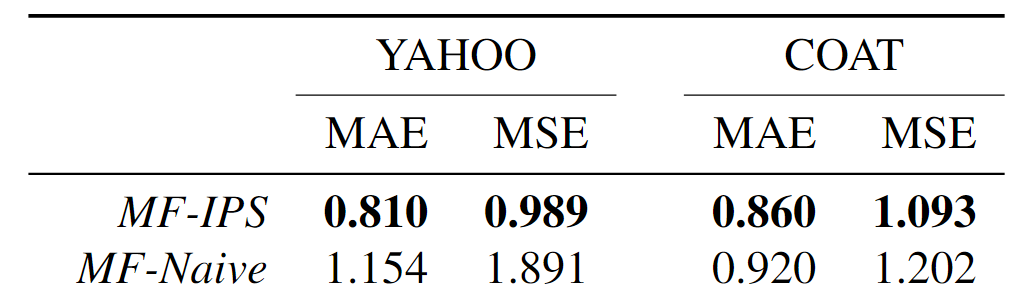
\includegraphics[width=\textwidth]{images/Chapter4/result.png}
    \caption{Kết quả thí nghiệm của bài báo trên tập test với bộ dữ liệu Yahoo và Coat}
    \label{fig:4_result}
\end{figure}



So với kết quả bài báo được thể hiện trong hình \ref{fig:4_result}. Thử nghiệm của nhóm em và kết quả của bài báo đều có cùng kết luận là phương pháp MF-IPS sẽ có kết quả trên tập test tốt hơn so với phương pháp MF thông thường, ngoài ra phương pháp MF-IPS sử dụng trên bộ dữ liệu Yahoo!R3 cải thiện được độ lỗi nhiều hơn so với phương pháp MF-IPS được sử dụng trên bộ dữ liệu Coat. Điều này có thể do bộ dữ liệu Yahoo!R3 bị lệch nhiều hơn bộ dữ liệu Coat hoặc cũng có thể do phương pháp ước lượng ma trận propensity bằng ''Naive Bayes'' sử dụng một phần thông tin được tiết lộ từ tập test nên kết quả thu được tốt hơn so với phương pháp ''Logistic Regression''. 

Tiếp theo, nhóm em sẽ tiến hành các thí nghiệm để làm rõ những vấn đề trên.

\section{Ảnh hưởng của việc dữ liệu bị thiên lệch tới việc học của MF và MF-IPS}
\subsection{Mức độ cải thiện của MF-IPS với MF khi học trên tập COAT với tập YAHOO}
\subsubsection{Mức độ thiên lệch của tập dữ liệu Coat và tập dữ liệu Yahoo}
Ta biết rằng bộ dữ liệu Coat và bộ dữ liệu Yahoo!R3 là những tập dữ liệu với tập test là MCAR trong khi tập training của chúng bị lệch. Nhóm em có tiến hành so sánh độ lệch của tập training với tập test trên hai bộ dữ liệu bằng độ đo KL - div hay còn gọi là độ đo ``Kullback-Leibler divergence'' tương tự như \cite{saito2020asymmetric}, giá trị của độ đo này càng lớn chứng tỏ tập training và tập test càng có phân phối khác biệt nhau. Cụ thể, các kết quả nhóm chúng em thu được như sau: 
\begin{itemize}
    \item Đối với tập dữ liệu Coat, giá trị của độ đo KL - div là 0.049, phân phối của nó được thể hiện trong hình \ref{fig:4_1_coat}.
    \item Đối với tập dữ liệu Yahoo, giá trị của độ đo KL - div là 0.469, phân phối của nó được thể hiện trong hình \ref{fig:4_2_yahoo}.
\end{itemize}

\begin{figure}[h]
    \centering
    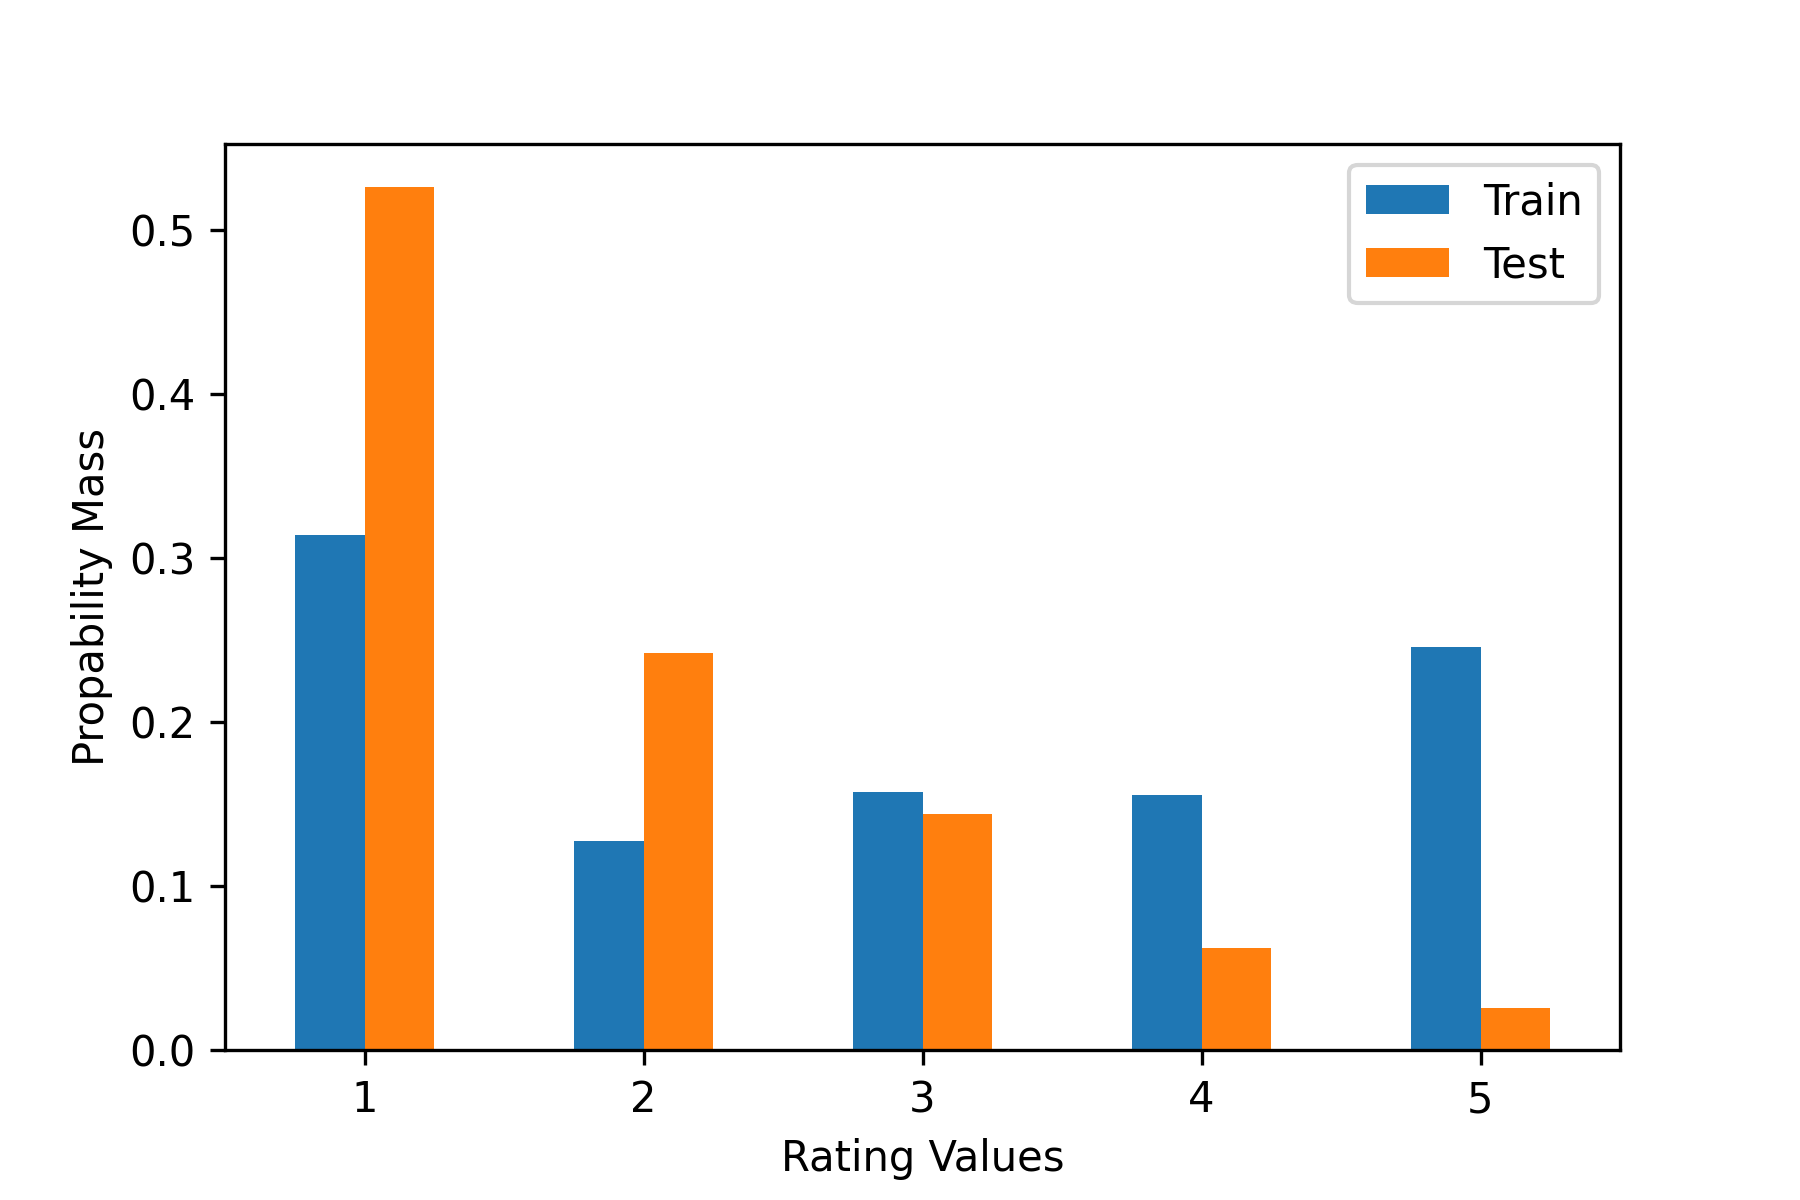
\includegraphics[width=\textwidth]{images/Chapter4/Diff_yahoo.png}
    \caption{Phân phối dữ liệu của tập training và tập test trên bộ dữ liệu Yahoo.}
    \label{fig:4_2_yahoo}
\end{figure}

\begin{figure}[h]
    \centering
    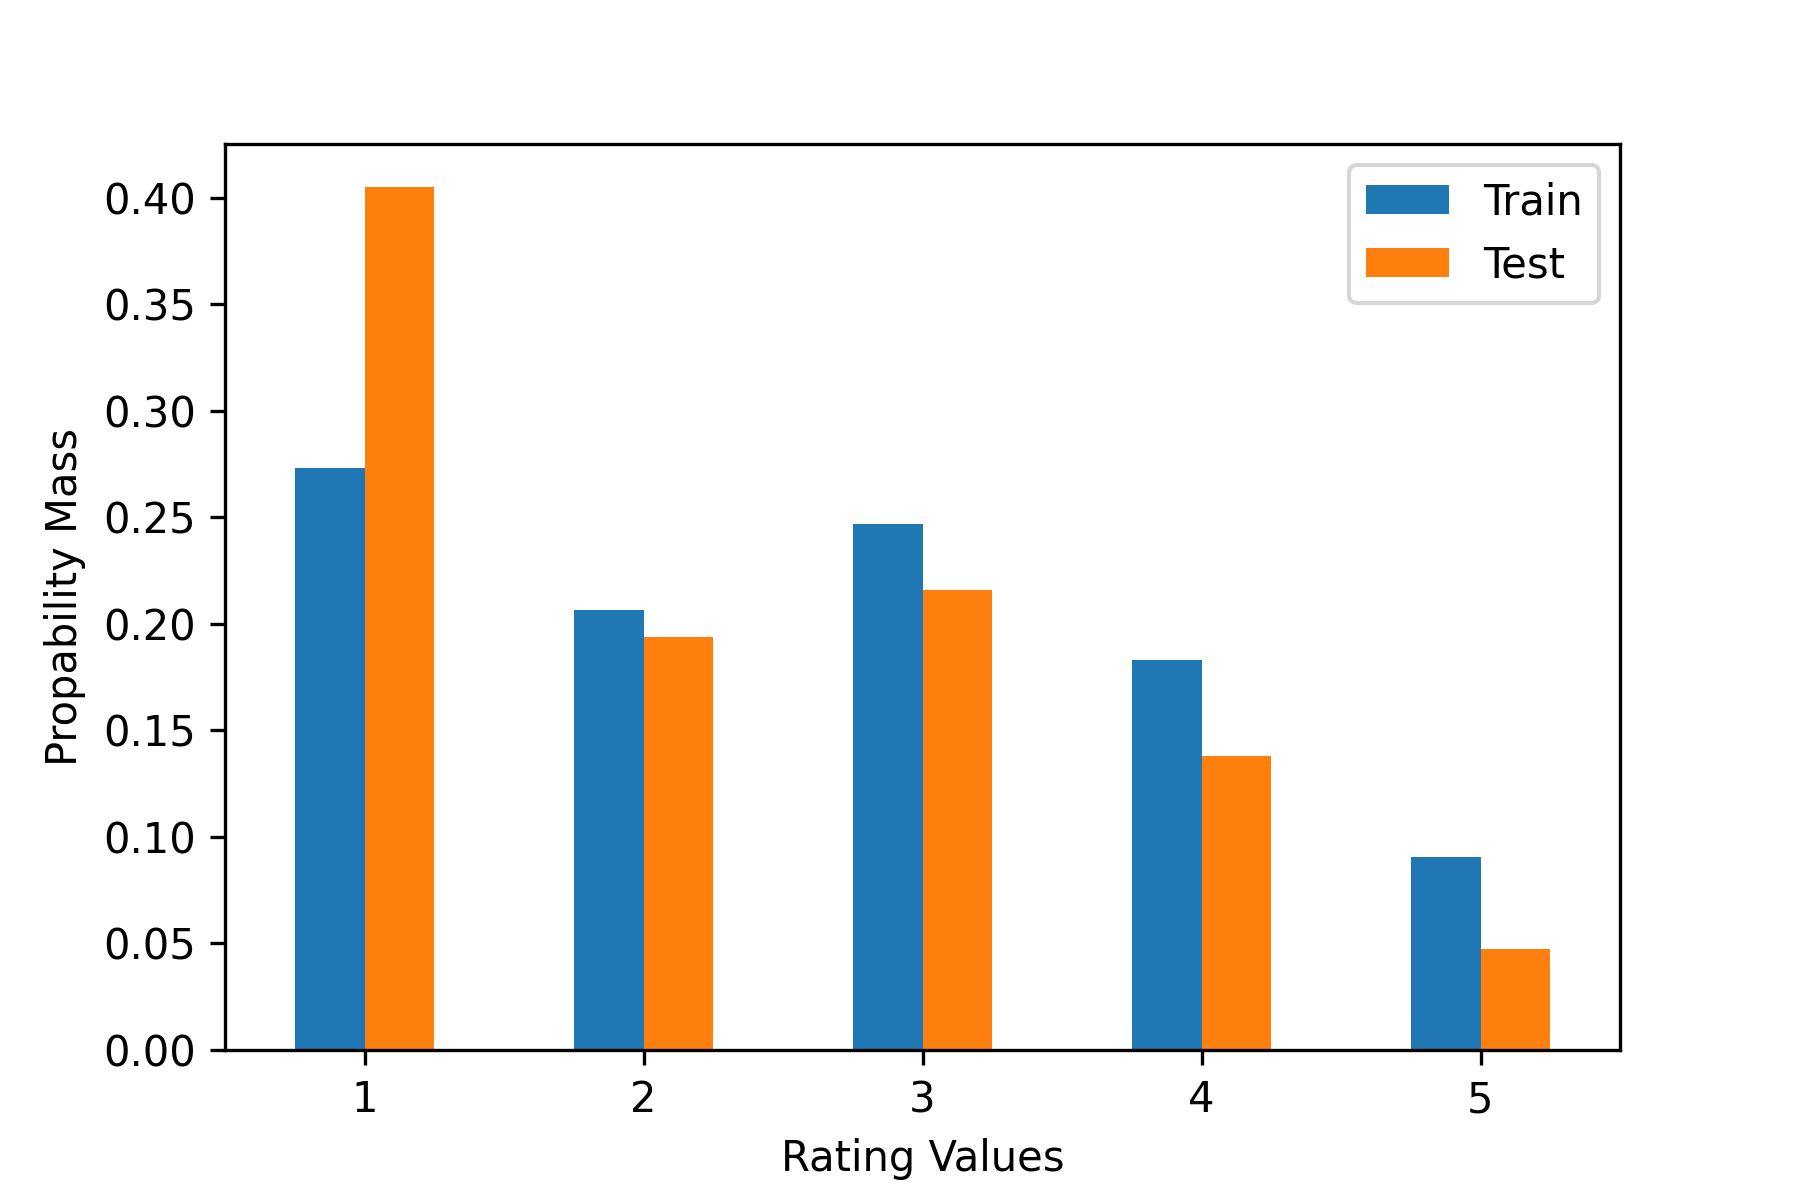
\includegraphics[width=\textwidth]{images/Chapter4/Diff_coat.png}
    \caption{Phân phối dữ liệu của tập training và tập test trên bộ dữ liệu Coat.}
    \label{fig:4_1_coat}
\end{figure}
Qua hình \ref{fig:4_2_yahoo}, hình \ref{fig:4_1_coat} và kết quả của độ đo KL - div ta có thể thấy chênh lệch về phân phối dữ liệu trong tập training và tập test của tập Yahoo lớn hơn tập Coat rất nhiều. Điều này có nghĩa là mức độ thiên lệch trong tập dữ liệu Yahoo cao hơn tập dữ liệu Coat nhiều, làm cho độ hiệu quả của phương pháp MF-IPS khi so với phương pháp MF sẽ được thể hiện nổi bật hơn ở trong tập Yahoo. Trong thí nghiệm tiếp theo nhóm em sẽ cho thấy rõ vấn đề này.
\subsubsection{Cách tiến hành}
Để biết được hiệu quả của phương pháp MF-IPS so với với phương pháp MF thông thường, nhóm em tiến hành thí nghiệm phương pháp MF-IPS và MF truyền thống trên cả hai bộ dữ liệu Coat và Yahoo. Để công bằng nhóm em sẽ sử dụng cùng một phương pháp ước lượng ma trận propensity đó là ``Naive bayes'' vì bộ dữ liệu Yahoo!R3 không có thông tin về người dùng - sản phẩm để thực hiện phương pháp ``Logistic regression''. Sau đó hai mô hình sẽ đánh giá độ lỗi MSE trên 95\% dữ liệu tập test và 5\% dữ liệu tập test còn lại sẽ được sử dụng để ước lượng propensity thông qua phương pháp ``Naive bayes''.
\subsubsection{Kết quả}
Bảng \ref{table:yahoo_coat_NB} cho thấy kết quả thí nghiệm của nhóm chúng em về độ lỗi MSE của 2 phương pháp MF và MF-IPS (với propensity được ước lượng thông qua ``Naive bayes'') trên 2 tập dữ liệu Yahoo và Coat.

\begin{table}[h]
    \centering
    \begin{tabular}{ccc}
    \hline
     & Yahoo & Coat \\ \hline
    MF-IPS & 0.976 & 1.080 \\
    MF & 1.899 & 1.197
    \end{tabular}
    \caption{Độ lỗi MSE của phương pháp MF và MF-IPS trên 2 tập dữ liệu Coat và Yahoo. Trong đó IPS được ước lượng thông qua ``Naive bayes''.}
    \label{table:yahoo_coat_NB}
\end{table}

Có thể thấy độ lỗi của phương pháp MF-IPS thấp hơn độ lỗi của phương pháp MF trên cả 2 tập dữ liệu Coat và Yahoo. Đặc biệt, tập dữ liệu Yahoo có mức độ thiên lệch dữ liệu nhiều hơn làm cho mức độ cải thiện của MF-IPS so với MF lớn hơn nhiều khi so sánh với mức độ cải thiện trên tập Coat.

\subsection{Mức độ cải thiện của MF-IPS với MF khi học trên tập MovieLens giả lập với mức độ thiên lệch của dữ liệu giảm dần}
\subsubsection{Tập MovieLens 100k giả lập}
\label{subsubsection:MovieLens}
Như đã trình bày ở phần trước, ở thí nghiệm này nhóm chúng em sẽ tiến hành thí nghiệm trên tập dữ liệu MovieLens 100k. Vì thí nghiệm này yêu cầu kiểm soát được mức độ thiên lệch của dữ liệu, nên nhóm chúng em sẽ tiến hành tạo một tập dữ liệu MovieLens~100k giả lập. 

Tập dữ liệu MovieLens~100k giả lập sẽ được tạo bằng cách sử dụng mô hình MF được huấn luyện trên toàn bộ tập dữ liệu MovieLens 100k, để điền toàn bộ giá trị còn thiếu trong ma trận tương tác giữa người dùng và sản phẩm MovieLens~100k. Với [$p_1, p_2, p_3, p_4, p_5$] là phân bố của dữ liệu trong tập MovieLens~100k giả lập, $p_1$ là tỉ lệ đánh giá 1 trong toàn bộ dữ liệu và tương tự với các đánh giá còn lại, thì phân bố dữ liệu sau khi hoàn thành ma trận giả lập là [$0.001, 0.027, 0.601, 0.364, 0.007$]. Có thể thấy các đánh giá trong ma trận giả lập này bị lệch nghiêm trọng, với số lượng đánh giá 3 và 4 chiếm số lượng rất lớn khi so với các đánh giá 1, 2 và 5. Điều này rất vô lý trong thực tế, vì vậy nhóm chúng em tiến hành điều chỉnh lại ma trận giả lập này tuân theo phân bố dữ liệu của tập test trong tập Yahoo!R3 là [$0.526, 0.242, 0.144, 0.062, 0.026$].

Ngoài ra, dữ liệu quan sát được sẽ được ước lượng như sau: Với các đánh giá 4 và 5, propensity để quan sát được các đánh giá này $k$. Đối với các đánh giá < 4, propensity để quan sát được các đánh giá này là $k\alpha^{4-r}$, với $r$ là các đánh giá và $\alpha \in [0,1]$ là tham số điều chỉnh mức độ thiên lệch dữ liệu. Với mỗi $\alpha$. $k$ được đặt sao cho số lượng dữ liệu quan sát được chỉ chiếm 5\% trên toàn bộ ma trận. Bằng cách thay đổi giá trị $\alpha$, chúng ta có thể thay đổi được mức độ thiên lệch dữ liệu. Khi $\alpha = 1$ dữ liệu sẽ được phát sinh hoàn toàn ngẫu nhiên theo phân phối đều (vì khi đó propensity của toàn bộ đánh giá đều bằng $k$). Khi $\alpha \rightarrow 0$ thì dữ liệu quan sát được chỉ chứa các giá trị 4 và 5 (vì khi đó propensity của các đánh giá 1,2 và 3 bằng 0). Lưu ý là với $\alpha = 0.25$ thì phân bố của dữ liệu quan sát được sẽ giống với phân bố của dữ liệu MovieLens 100k ban đầu ([0.06, 0.11, 0.27, 0.35, 0.21] trong tập dữ liệu gốc và [0.06, 0.10, 0.25, 0.42, 0.17] trên tập dữ liệu quan sát được)

\subsubsection{Cách tiến hành}
Sau khi có bộ dữ liệu quan sát được ta sẽ tiến hành huấn luyện 2 mô hình MF và MF-IPS trên tập dữ liệu này. Hai mô hình này sẽ được cross-validation để chọn tham số $\lambda$ khác nhau và tham số $d$ sẽ được cố định với $d = 20$. Ta sẽ tiến hành thay đổi giá trị $\alpha$ từ [0.0625, 0.125, 0.25, 0.5, 1] để điều chỉnh mức độ thiên lệch dữ liệu trên tập dữ liệu quan sát được được sử dụng để huấn luyện mô hình. Tập dữ liệu quan sát được sẽ được lấy từ tập dữ liệu MovieLens 100k giả lập tuân theo propensity của mỗi đánh giá, sao cho dữ liệu quan sát được chỉ chiếm 5\% tập dữ liệu MovieLens 100k giả lập.
\subsubsection{Kết quả}
Hình \ref{fig:4_movielens} mô tả kết quả thu được của nhóm em với độ lỗi MSE trên 2 mô hình MF và MF-IPS khi tiến hành thay đổi mức độ thiên lệch dữ liệu bằng cách thay đổi giá trị của $\alpha$.
\begin{figure}[h]
    \centering
    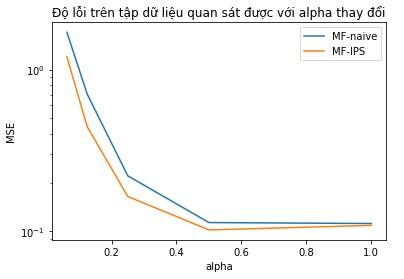
\includegraphics{images/Chapter4/movielens.jpg}
    \caption{Hình ảnh minh họa sự cải thiện về độ lỗi của MF và MF-IPS khi thay đổi mức độ thiên lệch của dữ liệu}
    \label{fig:4_movielens}
\end{figure}
% \begin{table}[h]
%     \centering
%     \begin{tabular}{|c|c|c|}
%     \hline
%     alpha & MF & MF-IPS \\ \hline
%     0.0625 & 1.932 & 1.098 \\ \hline
%     0.125 & 0.843 & 0.398 \\ \hline
%     0.25 & 0.248 & 0.153 \\ \hline
%     0.5 & 0.113 & 0.097 \\ \hline
%     1 & 0.108 & 0.108 \\ \hline
%     \end{tabular}
%     \caption{Độ lỗi MSE của hai mô hình MF và MF-IPS khi học trên tập MovieLens giả lập với mức độ thiên lệch của dữ liệu giảm dần.}
%     \label{table:4_movielens}
% \end{table}

Khi $\alpha$ nhỏ mức độ thiên lệch của dữ liệu cao (trong dữ liệu quan sát được đa phần chỉ chứa điểm đánh giá 4 và 5) thì độ lỗi trên 2 mô hình MF và MF-IPS rất cao. Mặc dù vậy, độ lỗi của mô hình MF-IPS vẫn có độ lỗi thấp hơn nhiều mô hình MF truyền thống. 

Khi $\alpha$ lớn mức độ thiên lệch dữ liệu của dữ liệu giảm dần (phân phối của các điểm đánh giá đều nhau hơn)
độ lỗi trên 2 mô hình này có sự cải thiện đáng kể và gần như xê xích nhau không nhiều. Mặc dù vậy mô hình MF-IPS vẫn cho độ lỗi thấp hơn mô hình MF. 

Tóm lại, khi dữ liệu bị thiên lệch nhiều phương pháp MF-IPS đã cho thấy độ hiệu quả của nó trong việc kiểm soát sự thiên lệch và cho kết quả cải thiện đáng kể trên tập dữ liệu bị thiên lệch này. Mặt khác, khi dữ liệu không bị thiên lệch (dữ liệu được phát sinh theo phân phối đều) phương pháp MF-IPS sẽ cho kết quả giống với phương pháp MF truyền thống, bởi vì lúc này dữ liệu không còn bị thiên lệch nên propensity của nó là như nhau trong mọi trường hợp làm cho MF và MF-IPS lúc này không có gì khác nhau.

\section{Ảnh hưởng của việc ước lượng ma trận propensity tới việc học của MF-IPS}
Trong phần này, nhóm em sẽ thiết kế các thí nghiệm để làm rõ ảnh hưởng của việc ước lượng ma trận propensity đến việc học của MF-IPS. Việc học của MF-IPS có thể bị ảnh hưởng bởi hiệu quả của việc ước lượng ma trận propensity, ta sẽ tiến hành xem xét mức độ hiệu quả của việc ước lượng ma trận propensity thông qua hai thiết lập sau:
\begin{itemize}
    \item Phương pháp ước lượng sẽ ảnh hưởng đến hiệu quả của việc ước lượng. Do đó nhóm sẽ tiến hành ước lượng ma trận propensity bằng cả phương pháp ``Logistic Regression'' và phương pháp ``Naive Bayes'' trên cùng bộ dữ liệu Coat, vì chỉ bộ dữ liệu này mới chứa thông tin của người dùng và sản phẩm để có thể tiến hành ước lượng ma trận propensity bằng phương pháp ``Logistic Regression''. 
    \item Khi sử dụng phương pháp ``Naive Bayes'' để ước lượng lượng ma trận propensity, số lượng mẫu MCAR được sử dụng có thể ảnh hưởng đến hiệu quả của việc ước lượng này và từ đó, ảnh hưởng đến quá trình học của MF-IPS.
\end{itemize}

\subsection{So sánh mức độ cải thiện của MF-IPS với MF bằng các phương pháp ước lượng ma trận propensity khác nhau}
Như đã trình bày ở trên, thí nghiệm này nhóm em sẽ sử dụng bộ dữ liệu Coat.
Với phương pháp ước lượng ma trận bằng propensity bằng ``Naive Bayes'', nhóm em sẽ sử dụng 5\% của tập test làm mẫu MCAR và chỉ đo độ lỗi của việc học MF-IPS trên 95\% còn lại của tập test. Với phương pháp ước lượng ma trận propensity bằng phương pháp ``Logistic Regression'', nhóm sẽ sẽ sử dụng thông tin của người dùng và sản phẩm để ước lượng. Để công bằng, nhóm cũng sẽ đo độ lỗi MF-IPS trên cùng một tập test được sử dụng bên trên. Ngoài ra nhóm cũng sử dụng phương pháp MF thông thường và dĩ nhiên cũng sẽ đo lại độ lỗi trên cùng một tập test để xem xét mức độ cải thiện của MF-IPS với MF bằng các phương pháp ước lượng ma trận propensity khác nhau. Kết quả mà nhóm em thu được như sau:

\begin{table}[h]
\centering
\begin{tabular}{|c|c|c|}
\hline
\multicolumn{1}{|l|}{} & MAE             & MSE             \\ \hline
MF                     & 0.9138          & 1.1973          \\ \hline
MF-IPS-LR              & 0.9037          & 1.1967          \\ \hline
MF-IPS-NB              & \textbf{0.8529} & \textbf{1.0795} \\ \hline
\end{tabular}
    \caption{Độ lỗi MSE và MAE của hai mô hình MF và MF-IPS với hai phương pháp ước lượng ma trận propensity khác nhau trên tập dữ liệu Coat.}
    \label{table:4_approach_estimate}
\end{table}

Bảng \ref{table:4_approach_estimate} cho ta thấy rằng phương pháp ước lượng ma trận propensity có ảnh hưởng đáng kể đến quá trình học của MF-IPS. Phương pháp ``Naive Bayes'' cho kết quả ước lượng tốt hơn phương pháp ``Logistic Regression'' vì theo như ví dụ ban đầu và theo nghiên cứu của Hu Nan \cite{bias_2017}, giá trị của mỗi đánh giá sẽ phần lớn quyết định khả năng đánh giá đó xuất hiện, hơn nữa việc sử dụng được phần nào phân phối của tập test cũng sẽ làm tăng hiệu quả của phương pháp ước lượng mà trận propensity bằng ``Naive Bayes''.

\subsection{So sánh mức độ cải thiện của MF-IPS với MF khi ước lượng ma trận propensity bằng ``Naive Bayes'' với số lượng dữ liệu MCAR khác nhau}
Ở thí nghiệm này, nhóm em sẽ sử dụng phương pháp ``Naive Bayes'' để ước lượng ma trận propensity. Tuy nhiên nhóm chỉ đo độ lỗi trên 90\% của tập test, phần còn lại sẽ được sử dụng làm mẫu MCAR cho quá trình ước lượng ma trận propensity, lượng tập test được tiết lộ lần lượt sẽ là [0.5\%, 1\%, 5\%, 10\%]. Nhóm em tiến hành thử nghiệm và kết quả thu được như hình \ref{fig:4_percent}, trong đó vùng bóng mờ là khoảng tin cậy 95\% trong 30 lần thử nghiệm.

\begin{figure}[h]
    \centering
    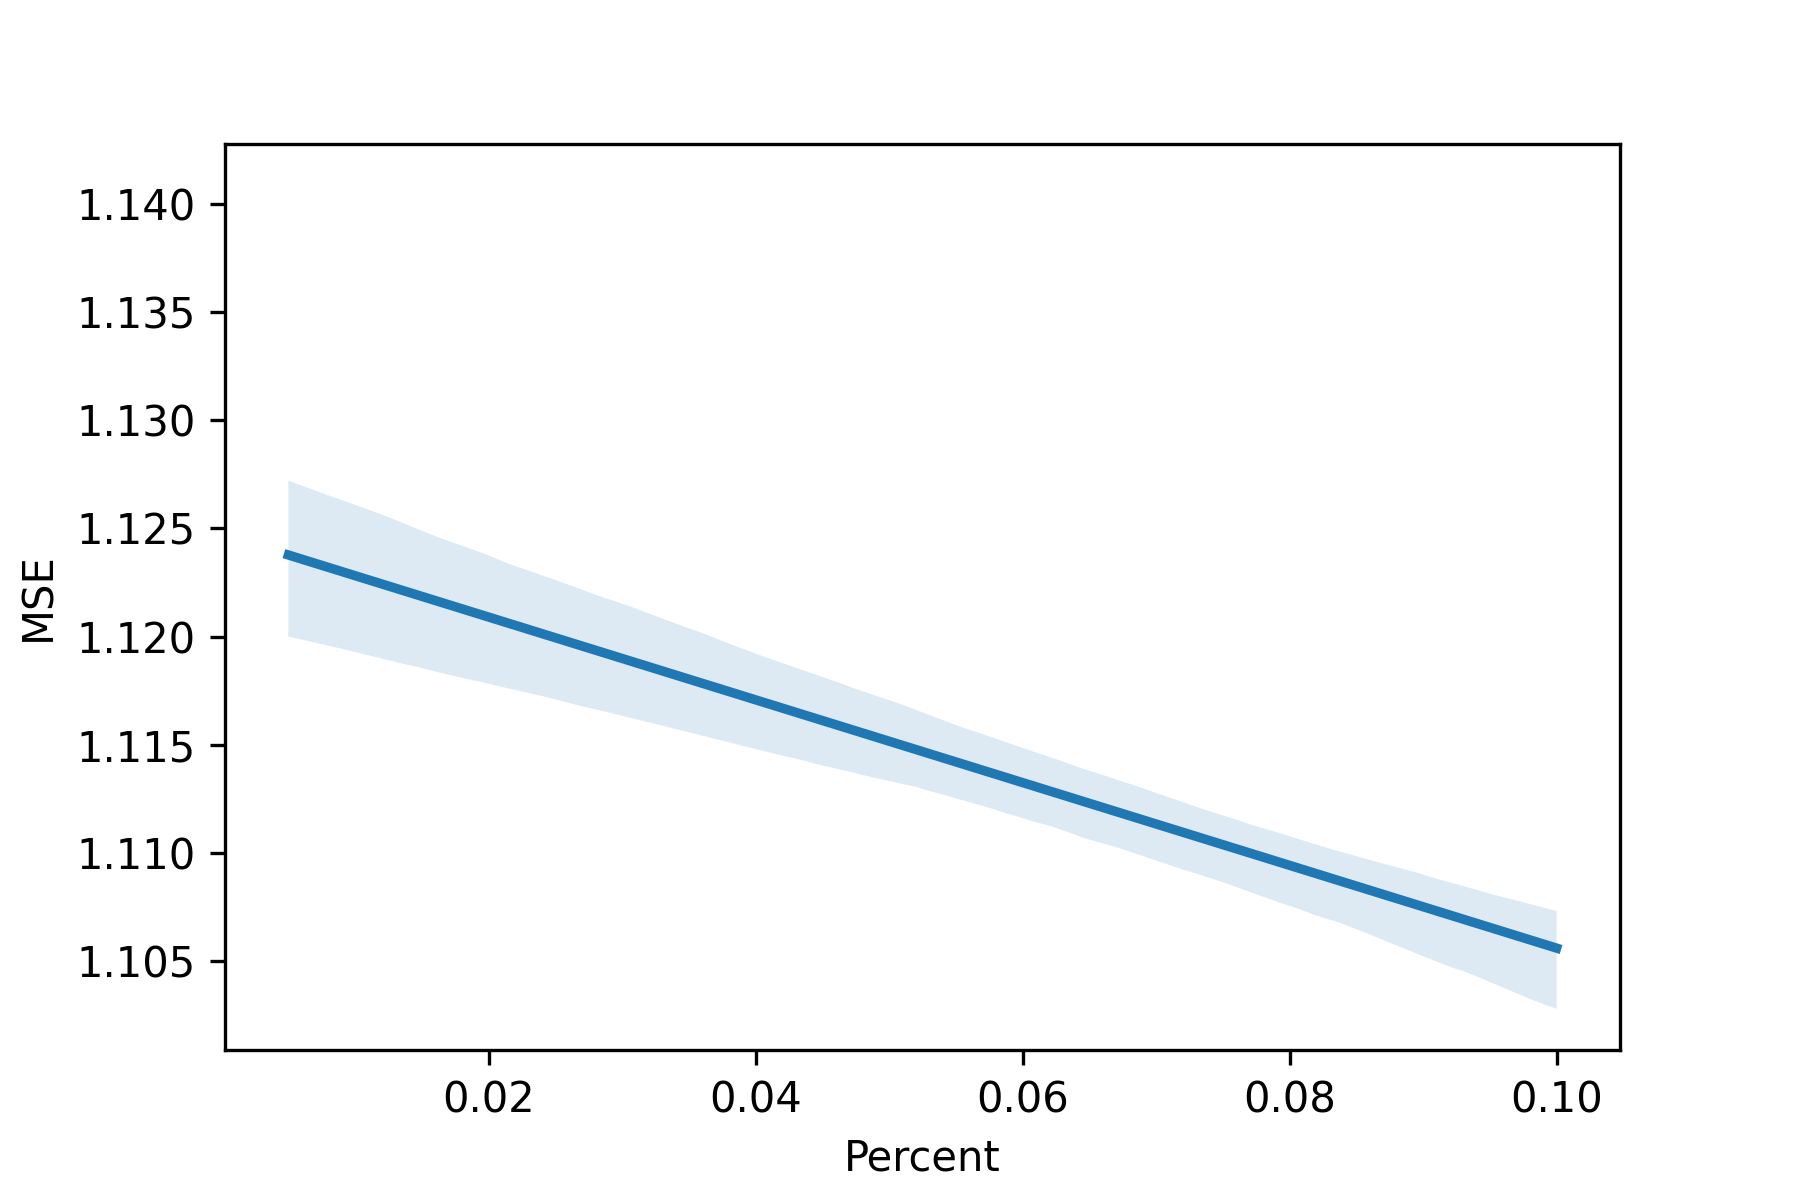
\includegraphics[width = \textwidth]{images/Chapter4/plot_percent1.png}
    \caption{Hình ảnh minh họa sự cải thiện về độ lỗi của MF và MF-IPS với lượng tiết lộ tập test khác nhau.}
    \label{fig:4_percent}
\end{figure}

Nhận xét: ta thấy rằng khi tăng lượng dữ liệu MCAR cho quá trình ước lượng ma trận propensity, việc học của MF-IPS sẽ có cải thiện. Điều này cũng khá dễ hiểu vì khi sử dụng càng nhiều lượng dữ liệu MCAR thì việc tính toán xác suất $P(Y=r)$ càng chính xác, giúp cho việc ước lượng propensity ít bị sai lệch hơn.

% \section{Đánh giá hiệu suất trên dữ liệu thế giới thực}
% \label{sec:4_performance}
% Mục tiêu: Nhằm đánh giá hiệu suất của mô hình ``Matrix factorization'' tiêu chuẩn (MF-Standard) và ``Matrix factorization'' (MF-IPS) sử dụng độ đo IPS trên 2 tập dữ liệu thế giới thực là Yahoo và Coat.

% Để sử dụng độ đo IPS trong việc huấn luyện mô hình ``Matrix Factorization'' trên 2 bộ dữ liệu ta tiến hành như sau:
% \begin{itemize}
%     \item Tập dữ liệu Yahoo: ta ước lượng ma trận propensity bằng phương pháp ``Naive Bayes''. Xác suất biên $P(Y=r)$ sẽ được tính toán thông qua 5\% của tập kiểm tra và 95\% còn lại sẽ được sử dụng để kiểm tra mô hình.
%     \item Tập dữ liệu Coat: ta ước lượng ma trận propensity bằng phương pháp ``Logistic Regression'' dựa trên hiệp biến của người dùng (giới tính, nhóm tuổi, vị trí và nhận thức về thời trang) và hiệp biến của sản phẩm (giới tính, loại áo khoác, màu sắc, và nó đã được khuyến mãi chưa). Mô hình ``Logistic Regression'' sẽ được huấn luyện bằng cách sử dụng tất cả các cặp hiệp biến của người dùng và sản phẩm làm các đặc trưng đầu vào, với nhãn là điểm đánh giá của người dùng cho các sản phẩm tương ứng; mô hình sẽ được cross-validation để tối ưu trên tập dữ liệu quan sát được do người dùng tự lựa chọn.
% \end{itemize}

% Kết quả: Bảng \ref{tab:4_performance} cho thấy hiệu suất của mô hình MF-IPS khi so sánh với MF-Standard, có thể thấy phương pháp MF-IPS có hiệu suất vượt trội hơn đáng kể khi so sánh với phương pháp thông thường.

% \begin{table}[h]
%     \centering
%     \begin{tabular}{|l|ll|ll|}
%     \hline
%     \multirow{2}{*}{} & \multicolumn{2}{c|}{Yahoo} & \multicolumn{2}{c|}{Coat} \\ \cline{2-5} 
%      & \multicolumn{1}{l|}{MAE} & MSE & \multicolumn{1}{l|}{MAE} & MSE \\ \hline
%     MF-IPS & \multicolumn{1}{l|}{0.810} & 0.989 & \multicolumn{1}{l|}{0.860} & 1.093 \\ \hline
%     MF-Standard & \multicolumn{1}{l|}{1.154} & 1.891 & \multicolumn{1}{l|}{0.920} & 1.202 \\ \hline
%     \end{tabular}
%     \caption{Hiệu suất trên 2 tập dữ liệu Yahoo và Coat}
%     \label{tab:4_performance}
% \end{table}

% \section{Dữ liệu thiên lệch ảnh hưởng đến việc đánh giá như thế nào?}
% \label{sec:4_evaluate}



% \section{Dữ liệu thiên lệch ảnh hưởng đến việc học như thế nào?}
% \label{sec:4_learning}
% \section{Tính mạnh mẽ của điểm propensity đã học không chính xác trong việc học và đánh giá mô hình như thế nào?}
% \label{sec:4_robust}

